\documentclass[../main/main.tex]{subfiles}

\newdate{date}{11}{12}{2019}


\begin{document}

\section{Functional partition function and coarse graining}
\marginpar{ \textbf{Lecture 17.} \\  \displaydate{date}. \\ Compiled:  \today.}

Since in proximity of the critical point the correlation length \( \xi  \) diverges, there is no point in which we can see small scales. It is convenient to rewrite the microscopic partition function as an effective partition function obtained by integrating out the degrees of freedom over regions of linear size \( l \gg a \) but still \( l \ll \xi  \). Indeed, a possible way to overcome the limitations of mean field theories can be the following: we could regard the profile of the order parameter \( m (\va{r}) \) to be the "degree of freedom" of our system and compute the partition function as a functional integral; in other words from the microscopic configuration of our system we can obtain \( m (\va{r}) \) with a \emph{coarse graining procedure} (we will immediately see what we mean by this) and then determine \( Z \) as a trace over all the possible configurations of our system, i.e. over all the possible forms of \( m(\va{r}) \):
%This \emph{coarse graining procedure} is formally given by
\begin{equation}
  Z = \Tr_{\{ S \}  } e^{- \beta \mathcal{H} [ \{ S \}  ]}
  = \int_{}^{} \mathcal{D}{\qty[m(\va{r})] } \qty[\sum_{ \substack{ \{ S \} \\ \text{compatible with the} \\ \text{profile } m(\va{r})}   }^{} e^{- \beta \mathcal{H} [ \{ S \}  ]] } ]
\end{equation}
where we traced over all the possible microscopic configurations \( \{ S \}   \) compatible with the order parameter profile \( m(\va{r}) \).
Let us define the effective Hamiltonian \( \mathcal{H}_{eff} \):
\begin{equation}
\sum_{ \substack{ \{ S \} \\ \text{compatible with the} \\ \text{profile } m(\va{r})}   }^{} e^ {- \beta \mathcal{H} [ \{ S \}  ]}
= e^{-\beta \mathcal{H}_{eff} (m (\va{r}))}
\label{eq:17_7}
\end{equation}
How, in pratice, can we perform the coarse graining procedure and obtain \( \mathcal{H}_{eff} \)?
We therefore must understand how to determine \( m(\va{r}) \); the idea of coarse graining procedures is the following: for a given microscopic configuration \( \{ S \}   \)  we average the order parameter \( m(\va{r}) \)  over sufficiently wide "blocks", i.e. portions of the system with linear dimension \( l \) much greater than its microscopic scale, which we call \( a \) (in the case of the Ising model, for example, \( a \)  can be taken as the lattice constant), but still microscopic and in particular much smaller than the correlation length \( \xi \), so that the order parameter is uniform in every block. In other words, coarse graining a system means dividing it into cells of linear dimension \( l \),  with \( l \) such that:
\begin{equation}
  a \ll l \ll \xi (T) < L
  \label{eq:17_1}
\end{equation}
(\( L \)  being the linear dimension of our system) and averaging the order parameter  \( m(\va{r}) \).  This way we can obtain an expression for \( m(\va{r}) \) (since \( l \) is anyway microscopic with respect to the size of the system, so we can regard  \( \va{r} \) as a continuous variable).

\begin{remark}
Hence, we partition the configurations according to the magnetization profile. For example, if we have a configuration with half spin up and half down, we obtain a profile with 1 and -1.
\end{remark}

\section{Coarse graining procedure for the Ising model}
To make things more clear, let us see how the coarse graining procedure works for the Ising model. For instance, see the two dimensional system represented in Figure \ref{fig:17_1}, where we have many spins in each square in which the system is divided.

\begin{figure}[h!]
\centering
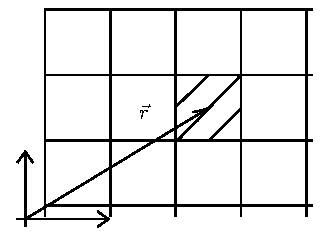
\includegraphics[width=0.5\textwidth]{../lessons/17_image/1.pdf}
\caption{\label{fig:17_1} Two dimensional system divided into cells with a huge number of spins.}
\end{figure}

If we call \( m_i = \expval{S_i}  \) the local magnetization at the \( i \)-th  and \( d \) the dimensionality of the system, once we have choosen the linear dimension \( l \), every "block" will have volume \( l^d \); we replace what it is inside every block of the system centered in \( \va{r} \), with the coarse grained magnetization:
\begin{equation}
  m_l (\va{r}) = \frac{1}{N_l} \sum_{i \in \va{r}}^{} S_i
\end{equation}
where \( N_l = (l/a)^d \) is the number of spins in each cell.

\begin{remark}
Since close to the critical point \( T_c \), we have that the correlation length diverges \( \xi \gg a \), we can always choose \( l \ll \xi  \) but still \( l \gg a \) such that the number \( N_l \) is large enough.
In this way, \( m(\va{r}) \) can be made to be a regular function of \( \va{r} \).
\end{remark}

Moreover, since it has been built as an average, \( m_l (\va{r}) \) does not fluctuate much on microscopic scales but varies smoothly in space. Of course, in general we need to specify \( l \) in order to determine \( m_l \), but the coarse graining procedure we are applying will be useful only if the final results are independent of \( l \)  (at least in the spatial scales considered).

\begin{remark}
In the reciprocal space (Fourier transform), the bound in Eq.\eqref{eq:17_1} implies the following cut off on the wave vector \( \va{q} \):
\begin{equation*}
  \abs{\va{q}} > \Lambda  = l^{-1}
\end{equation*}
Hence, this theory cannot develop ultraviolet divergences!
\end{remark}

We now must express the partition function in terms of \( m_l (\va{r}) \):
\begin{equation*}
  Z = \sum_{m_l (\va{r})}^{} \qty(\sum_{ \substack{ \{ S \} \\ \text{compatible with the} \\ \text{profile } m(\va{r})}   }^{} e^{-\beta \mathcal{H} ( \{ S \}  )}   )
 = \sum_{m_l(\va{r})}^{} e^{-\beta \mathcal{H}_{eff} [m(\va{r})]}
\end{equation*}
If \( m(\va{r}) \) is regular, the sum converges to a functional integral:
\begin{equation}
   Z_{GL} = \int_{}^{} \mathcal{D}  \qty[m_l (\va{r})]  e^{-\beta \mathcal{H}_{eff}[m(\va{r})]}
   \label{eq:17_8}
\end{equation}
so we must compute \( \mathcal{H}_{eff} [m(\va{r})] \).
First let us notice that Eq.\eqref{eq:17_7}:
\begin{equation*}
  \sum_{ \substack{ \{ S \} \\ \text{compatible with the} \\ \text{profile } m(\va{r})}   }^{} e^ {- \beta \mathcal{H} [ \{ S \}  ]}
  = e^{-\beta \mathcal{H}_{eff} (m (\va{r}))}
\end{equation*}
is proportional to the probability that the system displays a configuration with a profile \( m_l (\va{r}) \).

\subsection{Computation of \( \pmb{\mathcal{H}_{eff} [m(\va{r})]}\)}
 Since we now have a system made up of "blocks" this effective Hamiltonian will be composed of two parts: a bulk component relative to the single blocks and an interface component relative to the interaction between the blocks; let us consider them individually.

 \begin{itemize}
 \item \textbf{Bulk component}: suppose that every block of volume \( l^d \)  is separate from the rest of the system; inside every one of them the magnetization is uniform (since the linear dimension of the blocks is much smaller than the correlation length  \( l \ll \xi  \)), so we can use Landau theory for uniform systems. In the case of the Ising model, it led to the free energy:
\begin{equation*}
  \mathcal{L} = a t m^2 + \frac{\bar{b} }{4} m^4
\end{equation*}
The total bulk energy is thus obtained summing over all the blocks:
\begin{equation}
  \beta \mathcal{H}_{eff}^{bulk} [m] = \sum_{\va{r}}^{}  \bar{a} t m^2 (\va{r})+ \frac{\bar{b} }{2} m^4 (\va{r})
\end{equation}
Hence, the probability that the sistem displays a configuration with a profile \( m_l (\va{r}) \) is proportional to
\begin{equation}
  P^{cell} (m_l (\va{r})) \simeq e^{-\beta \mathcal{H}_{eff}^{bulk} (m (\va{r}))} = e^{ - \sum_{\va{r}}^{}  \bar{a} t m^2 (\va{r})+ \frac{\bar{b} }{2} m^4 (\va{r}) }
\end{equation}


\item \textbf{Interaction component:} we now must take into account the fact that adjacent blocks do interact. In particular, since as we have stated \( m \) does not vary much on microscopic scales, the interaction between the blocks must be such that strong variations of magnetization between neighbouring blocks is energetically unfavourable. If we call \( \va{\mu } \) a vector of magnitude \( l \) (\( \abs{\va{\mu }} =l  \)) that points from one block to a neighbouring one (see Figure \ref{fig:17_2}), the most simple analytic expression that we can guess for such a term can be a harmonic one:
\begin{equation}
  - \beta \mathcal{H}_{eff}^{int} =   \sum_{\va{r}}^{}  \sum_{\va{\mu }}^{}  \frac{\bar{k} }{2} \big( m (\va{r}+\va{\mu }) - m(\va{r})\big)^2 + O \qty( \qty(m (\va{r}+\va{\mu }) - m(\va{r}))^4 )
 \end{equation}
 (the factor \( 1/2 \) multiplying \( \bar{k}  \), just like the numeric factors multiplying \( \bar{a}  \)  and \( \bar{b}  \), have been inserted for future convenience). We can also think of this as a first approximation of a general interaction between the blocks, namely as the first terms of a Taylor expansion of the real interaction energy.

\begin{figure}[h!]
\centering
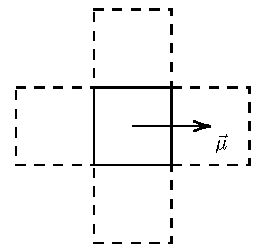
\includegraphics[width=0.3\textwidth]{../lessons/17_image/2.pdf}
\caption{\label{fig:17_2} Two dimensional system divided into block. The vector \( \va{\mu } \) points  from one block to a neighbouring one.}
\end{figure}

\end{itemize}

The total energy is thus obtained by summing the two terms. Now, since the linear dimension of the blocks \( l \)  is much smaller than the characteristic length \( L \) of the system we can treat \( \va{r} \)  as a continuous variable and thus substitute the sum over  \( \va{r} \) with an integral:
\begin{equation*}
  \sum_{\va{r}}^{}  \overset{\frac{l}{L} \ll 1}{\longrightarrow}   \frac{1}{l^d} \int_{}^{} \dd[d]{\va{r}}
\end{equation*}
(while the sum over \( \va{\mu } \) remains a sum, since for every \( \va{r} \)  there is only a finite number of nearest neighbours). Therefore:


\begin{itemize}
\item \textbf{Bulk component}:
\begin{equation}
  \beta \mathcal{H}_{eff}^{bulk} [m] =  \frac{1}{l^d} \int_{}^{} \qty( \bar{a} t m^2 (\va{r})+ \frac{\bar{b} }{2} m^4 (\va{r})  )  \dd[d]{\va{r}}
\end{equation}
Thus, if we now define for the sake of simplicity:
\begin{equation*}
  a \equiv \frac{\bar{a} }{l^d}, \quad b \equiv \frac{\bar{b} }{l^d}
\end{equation*}
we will have:
\begin{equation*}
  \beta \mathcal{H}_{eff}^{bulk} [m] = \int_{}^{} \qty( a t m^2 (\va{r})+ \frac{b }{2} m^4 (\va{r})  )  \dd[d]{\va{r}}
\end{equation*}


\item \textbf{Interaction component:}
\begin{equation}
  - \beta \mathcal{H}_{eff}^{int} =   \frac{1}{l^d} \int_{}^{}  \sum_{\va{\mu }}^{}  \frac{\bar{k} }{2} \big( m (\va{r}+\va{\mu }) - m(\va{r})\big)^2  \dd[d]{\va{r}}
 \end{equation}
 Keeping in mind that \( \abs{\va{\mu }}  = l \), the interaction term can be rewritten in terms of \( \va{\grad } m\):
\begin{equation*}
\begin{split}
\frac{1}{l^D} \int_{}^{}  \sum_{\va{\mu }}^{}  \frac{\bar{k} }{2} \big( m (\va{r}+\va{\mu }) - m(\va{r})\big)^2  \dd[d]{\va{r}} & = \frac{1}{l^{d-2}} \int_{}^{}
\frac{\bar{k} }{2} \sum_{\va{\mu }}^{}  \qty(\frac{m (\va{r}+\va{\mu }) - m(\va{r})}{l})^2 \dd[d]{\va{r}} \\
& = \frac{\bar{k} }{2l^{d-2}} \int_{}^{}
\sum_{\va{\mu }}^{}  \qty(\pdv{m}{ \chi  _ \mu } )^2 \dd[d]{\va{r}} \\
& \overset{\frac{a}{L} \ll \frac{l}{L} \ll 1}{\longrightarrow }  \int_{}^{}   \frac{k }{2} \qty(\va{\grad } m)^2  \dd[d]{\va{r}}
\end{split}
\end{equation*}
where we have called \( \chi _{\mu } \)  the components of \( \va{\mu } \) and we have rescaled the elastic constant by \( l^{d-2} \):
\begin{equation*}
  k \equiv  \frac{ \bar{k} }{l^{d-2}}
\end{equation*}
In this way the result is indipendent on \( l \).


\item \textbf{Total energy:}
\begin{equation}
  \beta \mathcal{H}_{eff} [m] = \int_{}^{}  \qty[a t m^2 (\va{r}) + \frac{b}{2} m^4 (\va{r}) + \frac{k}{2} \qty(\va{\grad } m (\va{r}))^2] \dd[d]{\va{r}}
\end{equation}
\end{itemize}

Therefore, the (functional) partition function of the system will be as in Eq.\eqref{eq:17_8}:
\begin{equation}
  Z_{GL} = \int_{}^{} \mathcal{D} \qty[m(\va{r})]   e^{ -\beta \mathcal{H}_{eff} [m(\va{r})]}
   = \int_{}^{} \mathcal{D} \qty[m(\va{r})]  e^{-   \int_{}^{}  \qty[a t m^2 (\va{r}) + \frac{b}{2} m^4 (\va{r}) + \frac{k}{2} \qty(\va{\grad } m (\va{r}))^2] \dd[d]{\va{r}}   }
\end{equation}
Let us now make a couple of considerations:
\begin{itemize}
\item If \( m(\va{r}) = m \) (uniform system) the energy of the system has the same structure of the one used in Landau theory.
\item The term proportional to \(   (\va{\grad } m (\va{r}))^2 \) is completely new but we could have introduced it intuitively to a Landau-like mean field functional, since the introduction of spatial variations in the order parameter has an energetic cost which must depend on how it varies in space, i.e. it depends on the gradient of \( m \). This term can be also added directly to the Landau theory by simply assuming that, whe \( m \rightarrow m(\va{r}) \) (one has to consider an additioned energy cost due to small variation of \( m \)).

Why we take \( (\va{\grad }m)^2  \) and not something else?
The choise is first of all a consequence of the isotropy of the system (all directions are equivalent). Since the system is isotropic and \( \mathbb{Z}^2 \)-invariant, we must use combinations of derivatives that are invariant under rotations and parity, and, among all the possible combinations, \(   (\va{\grad } m (\va{r}))^2 \) is the simplest one.

\end{itemize}

\begin{remark}
Let us consider the cases in which  \( m \rightarrow \va{m} \) (\( O(n) \) models); we have:
\begin{equation*}
  (\grad \va{m})^2 = \sum_{i=1}^{n} \sum_{\alpha =1}^{d}  \partial_ \alpha {m_i} \partial_ \alpha   {m_i}
\end{equation*}
Higher order terms are:
\begin{equation*}
  \qty(\grad ^2 \va{m})^2 =  \sum_{i=1}^{n} \sum_{\alpha =1}^{d} \sum_{\beta =1}^{d}
  \qty(\partial_ \alpha \partial_ \alpha {m_i}) \qty( \partial_ \beta \partial_ \beta {m_i})
\end{equation*}
and
\begin{equation*}
  \va{m}^2 \qty(\grad  \va{m})^2 =  \sum_{i=1}^{n} \sum_{j=1}^{n} \sum_{\alpha  =1}^{d} m_i m_i \partial_ \alpha {m_j} \partial_ \alpha {m_j}
\end{equation*}
In most cases it is sufficient to consider only the lowest order term.
\end{remark}

\subsection{Magnetic non-homogeneous field}
If there is also an external magnetic field
\begin{equation*}
  \va{h} ( \va{r}) = \beta \va{H} ( \va{r})
\end{equation*}
we must add to the Hamiltonian the term (Legendre transform):
\begin{equation*}
  - \int_{}^{}  \va{h} (\va{r}) \vdot \va{m} (\va{r}) \dd[d]{\va{r}}
\end{equation*}
so that the partition function becomes:
\begin{equation}
  Z_{GL} = \int_{}^{} \mathcal{D} \qty[m(\va{r})]  e^{-   \int_{}^{}  \qty[a t m^2 (\va{r}) + \frac{b}{2} m^4 (\va{r}) + \frac{k}{2} \qty(\va{\grad } m (\va{r}))^2 -  \va{h} (\va{r}) \vdot \va{m} (\va{r}) ] \dd[d]{\va{r}}   }
\end{equation}
which is a functional of \( m(\va{r}) \)  and \( \va{h}(\va{r}) \). As usual, all the thermodynamics of the system can be obtained from  \( Z_{GL} \), provided that now we take functional derivatives instead of usual derivatives.
Moreover, the free energy functional is defined as
\begin{equation}
  F [m,h] = \int_{}^{} \dd[d]{\va{r}} \qty[a t m^2 (\va{r}) + \frac{b}{2} m^4 (\va{r}) + \frac{k}{2} (\va{\grad }  m (\va{r}))^2 - h(\va{r})m(\va{r})]
  \label{eq:17_10}
\end{equation}


\subsection{Functional derivatives}
In the calculus of variations, a field of mathematical analysis, the functional derivative relates a change in a functional to a change in a function on which the functional depends. Functionals are usually expressed in terms of an integral of functions, their arguments, and their derivatives.

\begin{definition}{Functional derivative}{}
Given a manifold \( M \)  representing (continuous/smooth) functions \( h \)  (with certain boundary conditions etc.), and a functional \( G \)  defined as \( G: M \rightarrow \R \).
The functional derivative of \( G[h] \), denoted \( \delta G/\delta h \), is defined by
\begin{equation*}
  \int_{}^{}  \frac{\delta G }{\delta h}\qty(x) \Phi  (x) \dd[]{x}
= \lim_{\varepsilon \rightarrow 0} \frac{G \qty(h  +  \varepsilon \Phi  )- G(h)}{\varepsilon }
=\qty[ \dv{}{\varepsilon }  G[ h + \varepsilon \Phi  ]]_{\varepsilon =0}
\end{equation*}
where \( \Phi  \) is an arbitrary function.
In physics, it is common to use the Dirac delta function \( \delta (x-y) \) in place of a generic test function \( \Phi (x) \), for yielding the functional derivative at the point \( y \):
\begin{equation*}
\frac{\delta G [h(x)] }{\delta h(y)}  = \lim_{\varepsilon \rightarrow 0}
\frac{G [h(x) + \varepsilon \delta (x-y) ] - G[h(x)]}{\varepsilon }
\end{equation*}
or, in many dimensions:
\begin{equation}
\frac{\delta G [h(\va{r})] }{\delta h(\va{r'})}  = \lim_{\varepsilon \rightarrow 0}
\frac{G [h(\va{r}) + \varepsilon \delta (\va{r}-\va{r}') ] - G[h(\va{r})]}{\varepsilon }
\end{equation}
\subsubsection{Properties}
Like the derivative of a function, the functional derivative satisfies the following properties, where \( F[h] \) and \( G[h] \) are functionals:
\begin{itemize}
\item Linearity:
\begin{equation*}
  {\frac  {\delta (\lambda F+\mu G)[h ]}{\delta h (x)}}=\lambda {\frac  {\delta F[h ]}{\delta h (x)}}+\mu {\frac  {\delta G[h ]}{\delta h(x)}}
\end{equation*}
where \( \lambda\), \(\mu  \) are constants.
\item Product rule:
\begin{equation*}
{\frac  {\delta (FG)[h ]}{\delta h(x)}}={\frac  {\delta F[h ]}{\delta h (x)}}G[\rho ]+F[h]{\frac  {\delta G[h ]}{\delta h (x)}}
\end{equation*}
\item Chain rules:
if \( F \)  is a functional and \( G \)  another functional, then
\begin{equation*}
  \frac{\delta F[G[h]] }{\delta h(y)}  = \int dx \eval{\frac{\delta F[G]}{\delta G(x)}}_{G = G[h]} \cdot\frac {\delta G[h](x)} {\delta h(y)}
\end{equation*}
If \( G \)  is an ordinary differentiable function (local functional) \( g \), then this reduces to:
\begin{equation*}
   {\frac {\delta F[g( h )]}{\delta h(y)}}={\frac {\delta F[g( h)]}{\delta g[h (y)]}} \dv{g(h )}{ h(y)}
\end{equation*}
\end{itemize}
\end{definition}

Let us consider some examples.

\begin{example}{Functional derivative of a function}{}
A function can be written in the form of an integral like a functional. For example,
\begin{equation*}
  f(\va{r}) \equiv F[ f ] = \int f ( \va{r}') \delta^d(\va{r}-\va{r}')\dd[d]{\va{r}'}
\end{equation*}
Since the integrand does not depend on derivatives of \( f \), the functional derivative of \(   f(\va{r})  \)  is,
\begin{equation}
  \frac{\delta f (\va{r})}{\delta f (\va{r}')} \equiv \frac{\delta F}{\delta f (\va{r}')}
  =\pdv{}{f (\va{r}')}  \qty[ f ( \va{r}') \delta^d (\va{r}-\va{r}')] =  \delta^d (\va{r}-\va{r}')
  \label{eq:17_12}
\end{equation}

\end{example}

\begin{example}{Functional derivative of interaction component of \( \pmb{\mathcal{H}_{eff} } \)}{}
The functional derivative of the interaction component of \( \mathcal{H}_{eff} [m (\va{r})]\) is
  \begin{equation}
    \frac{\delta }{\delta m (\va{r})} \qty[ \int_{}^{}  \frac{k }{2} \qty(\va{\grad } m (\va{r}'))^2  \dd[d]{\va{r}'}     ]  =- k \qty(\va{\grad } ^2 m )
    \label{eq:17_9}
  \end{equation}
\end{example}
Taking into account the result Eq.\eqref{eq:17_9}, we have:
\begin{equation}
  \expval{m(\va{r})} = - \frac{\delta F}{\delta h (\va{r})} = - \frac{\delta \ln{Z[h]} }{\delta h (\va{r})}
\end{equation}
and one can show that the magnetic suscpetibility is
\begin{equation}
\begin{split}
  \chi  (\va{r},\va{r}') & = \frac{\delta ^2 F}{\delta h(\va{r}) \delta h(\va{r}')}
  = \beta ^{-1} \frac{\delta ^2 \ln{Z[h]} }{\delta h (\va{r}) \delta h (\va{r}')}\\
  & = \beta ^{-1} \qty[ \expval{m(\va{r}) m (\va{r}')} - \expval{m (\va{r})} \expval{m(\va{r}')}  ]
   = \beta ^{-1} G_c (\va{r},\va{r}')
\end{split}
\end{equation}
The problem is again try to approximate this term as much as we can. Let us do it.



\section{Saddle point approximation: Landau theory for non-homogeneous systems}
We can now compute \( Z \), as a first approach, using the saddle point approximation; as we will see this will reproduce a Landau-like mean field theory which will also take into account the presence of inhomogeneities. In particular thanks to the new term involving \( \va{\grad } m (\va{r}) \) we will be able to compute the fluctuation correlation function and so also to determine the critical exponents \( \eta  \) and \( \nu  \). Let us recall the results previously obtained:
\begin{equation*}
  Z_{GL} = \int_{}^{} \mathcal{D} \qty[m(\va{r})]  e^{-  \beta \mathcal{H}_{eff} [m (\va{r})]   + \int_{}^{} \va{h} (\va{r}) \vdot \va{m} (\va{r})  \dd[d]{\va{r}}   }
\end{equation*}
where \( h(\va{r}) = \beta H(\va{r}) \) and
\begin{equation*}
  \beta \mathcal{H}_{eff} [m] = \int_{}^{}  \qty[a t m^2 (\va{r}) + \frac{b}{2} m^4 (\va{r}) + \frac{k}{2} \qty(\va{\grad } m (\va{r}))^2] \dd[d]{\va{r}}
\end{equation*}
Therefore we approximate \( Z \) with the leading term of the integral, i.e. we must determine the function \( m_0 \)  that maximizes the exponent, namely minimizes:
\begin{equation}
  L (m,\va{\grad } m,h) =  \beta \mathcal{H}_{eff}   - \int_{}^{} \va{h}  \vdot \va{m}  \dd[d]{\va{r}} = \int_{}^{}  \qty[a t m^2  + \frac{b}{2} m^4 + \frac{k}{2} \qty(\va{\grad } m )^2 - \va{h}  \vdot \va{m} ] \dd[d]{\va{r}}
\end{equation}
 Let \( m_0 (\va{r}) \) be the profile for which \( L (m_0 (\va{r}), h (\va{r}) ) \) is minimum, then compute \( Z_{GL} \) as
\begin{equation}
  Z_{GL} [h] \overset{\substack{ \text{saddle} \\  \text{point} } }{\simeq } Z_{GL}^0 [h] = e^{- L [m_0 (\va{r})]}
\end{equation}
In order to find the minimum \( m_0 (\va{r}) \), one has to impose the stationarity condition of the functional \( L \): % with respect to \( m \):
% \begin{equation}
%   \eval{\frac{\delta L}{\delta m}}_{m_0} = 0
%   \label{eq:17_3}
% \end{equation}
\begin{equation}
  \delta L = 0
  \label{eq:17_3}
\end{equation}
Now, let us define \( \mathfrak{h} \) the integrand of \( \beta \mathcal{H}_{eff} \):
\begin{equation*}
  \mathfrak{h} = a t m^2 + \frac{b}{2} m^4 + \frac{k}{2} (\va{\grad } m)^2
\end{equation*}
By considering \( \delta L \) with respect to the variations \( \delta m \) and \( \delta (\grad m) \), one gets the equation of state
\begin{empheq}[box=\myyellowbox]{equation}
  h (\va{r}) = - \qty[\va{\grad } \qty(\pdv{ \mathfrak{h} }{(\va{\grad }m)} ) - \pdv{\mathfrak{h} }{m}  ]
  \label{eq:17_2}
\end{empheq}
Hence, by using the definition of \( \mathfrak{h} \), we obtain the state equation:
\begin{equation}
  h (\va{r}) = - k \va{\grad } ^2 m_0 (\va{r}) + 2 a t m _0 (\va{r}) + 2 b m_0^3 (\va{r})
   \label{eq:17_4}
\end{equation}
  this is the mean field solution of the Gibbs-Landau. It is more general than the one found before, indeed it has the additional term \( \va{\grad } \).
Let us note that:
\begin{itemize}
\item If \( h= 0 \): Eq.\eqref{eq:17_2} reduces to the \emph{Euler-Lagrange equation}
\begin{equation}
  \pdv{\mathfrak{h} }{m} = \va{\grad } \qty(  \pdv{\mathfrak{h}}{(\va{\grad } m)})
  \label{eq:17_11}
\end{equation}

\item If \( h (\va{r}) = h \) (homogeneous field) and \( m_0 (\va{r})=m_0 \): Eq.\eqref{eq:17_4} reduces to the equation of state of the Landau theory of uniform systems
\begin{equation*}
  h = 2 a t m_0 + 2 b m_0 ^3
\end{equation*}

\end{itemize}

 \begin{remark}
Moreover, note that a mean field theory of systems with spatial disomogeneity can start directly by considering the free energy functional defined in Eq.\eqref{eq:17_10}:
   \begin{equation*}
     F[m,h] = \int_{}^{}  \qty[a t m^2 (\va{r}) + \frac{b}{2} m^4 (\va{r}) + \frac{k}{2} (\grad m)^2 - h (\va{r}) m(\va{r})] \dd[d]{\va{r}}
   \end{equation*}
\end{remark}





\begin{example}{Show relation \eqref{eq:17_11}}{}
Let us consider the case \( h=0 \), we want to obtain the Euler-Lagrange equation:
\begin{equation*}
  \pdv{\mathfrak{h} }{m} = \va{\grad } \qty(  \pdv{\mathfrak{h}}{(\va{\grad } m)})
\end{equation*}
In order to do that, we define
  \begin{equation*}
    L [m, \va{\grad } m,h] = \int_{}^{}  \mathcal{L} (m, \va{\grad } m,h)\dd[d]{\va{r}}
  \end{equation*}
Supposing \( h=0 \)  and looking for the variation of \( L \) with respect to the variations of \( m,\, \delta m \),  and the variation of \( \va{\grad } m, \, \delta (\va{\grad } m) \), we have:

  \begin{equation*}
  \begin{split}
  \delta L [m, \va{\grad } m,0]  &=  \int_{}^{} \mathcal{L} (m+\delta m, \va{\grad } m + \delta (\va{\grad } m))  \dd[d]{\va{r}} - \int_{}^{}  \mathcal{L} (m,\va{\grad } m) \dd[d]{\va{r}}   \\
  & = \int_{}^{}  \qty[\mathcal{L} (m+\delta m, \va{\grad } m + \delta ( \va{\grad } m)) - \mathcal{L} (m, \va{\grad } m)] \dd[d]{\va{r}} \\
  & = \int_{}^{} \qty[\pdv{\mathcal{L}}{m} \delta m +
  \mathcolorbox{red!30}{ \underset{f}{\pdv{\mathcal{L}}{(\va{\grad } m)} } \underset{g'}{\delta (\va{\grad } m) }  }
  ] \dd[d]{\va{r}}
  \end{split}
  \end{equation*}
  where in the last step we did a Taylor expansion around \( (m, \va{\grad } m) \).
  We now integrate by parts (i.e. \( \int_{}^{} f g' = fg - \int_{}^{} f'g     \)) the red term, obtaining
  \begin{equation*}
  \begin{split}
  \delta L &= \int_{}^{} \qty[\pdv{\mathcal{L}}{m} \delta m - \va{\grad } \pdv{\mathcal{L}}{(\va{\grad } m)} \delta m ] \dd[d]{\va{r}} +
  \mathcolorbox{blue!20}{\int_{}^{}  \qty[\pdv{\mathcal{L}}{\va{\grad } m} \delta m ] \dd[d]{\va{r}} }
  \\
   & = \int_{}^{}  \qty[\pdv{\mathcal{L}}{m} \delta m - \va{\grad } \pdv{\mathcal{L}}{(\va{\grad } m)} \delta m ]\dd[d]{\va{r}} + \mathcolorbox{blue!20}{\int_{V}^{}  \va{\grad } \qty[\pdv{\mathcal{L}}{\va{\grad } m} \delta m ] \dd[d]{\va{r}} }
  \end{split}
  \end{equation*}
  where for the blue term we have used the divergence theorem \( \int_{\partial{ \Omega }}^{} F = \int_{V}^{} \va{\grad } F     \). Moreover, the blue term vanishes at the boundary of the integration. Hence, we have
  \begin{equation*}
    \delta L = \int_{}^{} \delta m \qty[\pdv{\mathcal{L}}{m} - \va{\grad } \pdv{\mathcal{L}}{(\va{\grad } m)}  ]  \dd[d]{\va{r}}
  \end{equation*}

  The stationarity condition \( \delta L = 0 \) (Eq.\eqref{eq:17_3}) is true \( \forall \delta m \neq 0 \) if and only if the integrand is zero, thus we obtain the \emph{Euler-Lagrange equation}:
  \begin{equation*}
    \pdv{\mathcal{L}}{m} - \va{\grad } \qty(\pdv{\mathcal{L}}{(\va{\grad } m)} ) = 0
  \end{equation*}
  Hence, when \( h=0 \), we have \( \mathcal{L} \rightarrow  \mathfrak{h} \).

\end{example}





\section{Correlation function in the saddle point approximation for non-homogeneous systems}
\label{sec:17_1}
We can now proceed to compute the correlation function within our approximations. In order to do that, we take the (functional!) derivative of the state equation \eqref{eq:17_4} with respect to \( h (\va{r}') \). Remembering that
\begin{equation*}
  \chi _T (\va{r},\va{r}') = \frac{\delta m(\va{r})}{\delta h (\va{r}')}
\end{equation*}
and that from Eq.\eqref{eq:17_12}:
\begin{equation*}
  \frac{\delta h (\va{r})}{\delta h (\va{r}')} = \delta (\va{r}-\va{r}')
\end{equation*}
The functional derivative becomes
\begin{equation}
  \delta  (\va{r} - \va{r}')  = \frac{\delta h(\va{r})}{\delta m (\va{r})} \frac{\delta m(\va{r})}{\delta h (\va{r}')} = \qty[- k \va{\grad }^2 + 2 a t    + 6 b m_0^2 (\va{r}) ]   \chi _T (\va{r}-\va{r}')
\end{equation}
where we have assumed translational invariance (i.e. uniform systems).
Now, from fluctuation-dissipation theorem we know that:
\begin{equation*}
  G_c (\va{r}-\va{r}') = k_B T \chi _T (\va{r}-\va{r}')
\end{equation*}
so that
\begin{equation}
  \beta \qty[-k \va{\grad } ^2 + 2 a t + 6 b m_0 ^2 ] G_c (\va{r}-\va{r}') = \delta (\va{r}- \va{r}')
  \label{eq:17_5}
\end{equation}
Note that this means that the correlation function \(  G_c (\va{r}-\va{r}')\)  can be interpreted as the Green's function of the operator \( D \) written between the square brackets:
\begin{equation*}
  D \equiv - k \va{\grad } ^2 + 2 a t + 6 b m^2
\end{equation*}
the equation \eqref{eq:17_5} is also known as \emph{Fundamental Equation} and \( G_c (\va{r}- \va{r}') \)  as Fundamental Solution, or Green's function of the differential operator \( D \).

As said, in case of translationally invariant (i.e. uniform) systems, \( m \) is constant and equal to the equilibrium values given by the Landau theory for the Ising model; in particular, depending on the sign of \( t \) there are two possible situations:
% We now look for the solutions of \eqref{eq:17_5}.  We consider two cases, \( T > T_c \) and \( T < T_c \) and let \( h \rightarrow 0 \).
\begin{itemize}

\item Case \( t>0 \) (\( T > T_c \)): in this case the mean field solution is \( m (\va{r}) = m_0 = 0 \), so the last equation becomes:
\begin{equation}
  \qty(-k \grad ^2 + 2 a t ) G_c (\va{r}-\va{r}') = k_B T \delta (\va{r}-\va{r}')
  \label{eq:17_6}
\end{equation}
Defining:
\begin{equation*}
  \xi_> (t) \equiv  \qty(\frac{k}{2 a t })^{1/2}
\end{equation*}
this can be rewritten as:
\begin{equation*}
  \qty(-\grad ^2 + \xi _> ^{-2} (t)) G_c (\va{r}-\va{r}') = \frac{k_B T}{k} \delta (\va{r}-\va{r}')
\end{equation*}


\item Case \( t<0 \) (\( T < T_c \)): in this case the magnetization is:
\begin{equation*}
  m_0 = \pm \qty(-\frac{at}{b})^{1/2}
\end{equation*}
so the differential equation for \( G_c \) becomes:
\begin{equation}
  \qty(-k \grad ^2 - 4 a t ) G_c (\va{r}-\va{r}') = k_B T \delta (\va{r}-\va{r}')
\end{equation}
Defining:
\begin{equation*}
  \xi _{<} (t) \equiv \qty(- \frac{k}{4at})^{1/2}
\end{equation*}
this can be written as
\begin{equation*}
  \qty(-\grad ^2 + \xi _<^{-2} (t))G_c (\va{r}- \va{r}') = \frac{k_B T}{k} \delta (\va{r}- \va{r}')
\end{equation*}

\end{itemize}

We will shortly see that \( \xi _{>} \)  and \( \xi _{<} \)  are the expressions of the correlation length for \( T>T_c \)  and \( T<T_c \) , respectively. We can therefore see that in both cases we get:
\begin{equation}
  \xi \sim t^{-1/2} \quad \Rightarrow \nu  = \frac{1}{2}
\end{equation}
that is the mean field value of \( \nu  \)!

\begin{remark}
Since \( \nu = 1/2 \), the upper critical dimension of a critical point belonging to the Ising universality class is
\begin{equation*}
  d_c = \frac{2}{\nu } = 4
\end{equation*}
as previously anticipated.
\end{remark}

We have seen that for both the cases, \( t>0 \) and \( t<0 \),  the correlation function  can be obtained by solving the differential equation:
\begin{equation}
  \qty(- \grad ^2 + \xi ^{-2}) G_c (\va{r}-\va{r}') = \frac{k_B T}{k} \delta (\va{r}-\va{r}')
  \label{eq:17_13}
\end{equation}
which can be can be solved  with the Fourier transform and by using spherical coordinates. 



\end{document}
